
%(BEGIN_QUESTION)
% Copyright 2014, Tony R. Kuphaldt, released under the Creative Commons Attribution License (v 1.0)
% This means you may do almost anything with this work of mine, so long as you give me proper credit

Complete the table of values for this circuit:

$$\includegraphics[width=15.5cm]{i01178x01.eps}$$

\vfil 

\underbar{file i01178}
\eject
%(END_QUESTION)





%(BEGIN_ANSWER)

This is a graded question -- no answers or hints given!

%(END_ANSWER)





%(BEGIN_NOTES)

A recommended problem-solving strategy is to first re-draw the schematic in a "cleaner" form so we can better discern the series and parallel relationships.  A simple way to do this is to re-draw the schematic in such a way that all resistors are oriented in the same direction.  Here, I will show all resistors oriented horizontally:

$$\includegraphics[width=15.5cm]{i01178x03.eps}$$

Now that the circuit has been re-drawn, we can easily see that resistor $R_5$ has been shorted past by a length of wire and is therefore of no effect.  Likewise, we can see that resistors $R_1$ and $R_3$ are in parallel with each other, and that their parallel combination is in series with resistor $R_2$.  The calculations thus reflect full source voltage across resistor $R_4$ and across the series-parallel combination $R_2$ - - ($R_1$ // $R_3$).

$$\includegraphics[width=15.5cm]{i01178x02.eps}$$

%(END_NOTES)


